\documentclass{article}
% \documentclass{report}
\usepackage[utf8]{inputenc}
\usepackage{graphicx}

\title{TEMPLATE}
\author{Suki Yau}
\date{\today}

\usepackage{natbib}
\usepackage{graphicx}
\usepackage{booktabs}
\usepackage{multirow}
\usepackage{caption}
\usepackage{subcaption}
\usepackage{mwe}
\usepackage{textgreek}
\usepackage[table,xcdraw]{xcolor}
\usepackage[fleqn]{amsmath}
\usepackage[]{soul}
\usepackage{textgreek}
\usepackage{amsmath}

%verbatim packages
\usepackage{moreverb}


%matlab packages
\usepackage[T1]{fontenc}
\usepackage{bigfoot} % to allow verbatim in footnote
\usepackage[numbered,framed]{matlab-prettifier}
\usepackage{filecontents}

\let\ph\mlplaceholder % shorter macro
\lstMakeShortInline"

\lstset{
  style              = Matlab-editor,
  basicstyle         = \mlttfamily,
  escapechar         = ",
  mlshowsectionrules = true,
}


\graphicspath{ {./images/} }

\begin{document}

\lstset{language=Matlab}

\maketitle
% \begin{abstract}
%     abstract hdkvgfhjislf
% \end{abstract}

\newpage
\tableofcontents
\listoffigures

%% Include A3 posters at end of thesis
%% datavizcatalogue.com 
%% academic phrasebank website 
%% TIP: when captioning figures - if caption is really long, use square brackets around the start to shorten in the contents e.g [blah blah] blah blah blah blah 
%% Get orchid ID

\section{Introduction}
In this chapter, the previously characterised Surface Probe prototype \hl{indicated} a removable window is prone
to \hl{many issues}, and a particle window deposited straight onto the chip could both \hl{solve these issues}
and produce a higher sensitivity.

\subsection*{CMOS Digital Image Sensor}

How does it work

\begin{itemize}
\item Upgrade previously characterised window samples 
\item  -- why 
\item 
\item Goal: increased sensitivity -- hit OD 5, keep film thin 
\item Goal: increased robustness -- no longer removable window -- e beam 
\item Goal: Biocompatibility -- Al ox passivation layer 
\end{itemize}

\section{Material properties}

This section names important material paramters in deposition and their
relation to the final multilayer design. The understanding of those dependencies
is of importance for the final forming result obtained.

The Biocompatibility
The optical density 
The hardness/scratch test

\subsection{First layer}
theory of aluminium 

thermodynamics of nucleaus formation

crystal growth 

aluminium is not biocompatible so a passivation layer is needed to protect 

aluminium oxide is chosen as it will develop a native oxide that will adhere 
\subsection{Passivation layer}

\section{Deposition techniques}

what do we want? nanometer layers of material 

most popular method?

must have clean substrate to reduce pinhole and hillocks ((WHY)) + HOW does it cause pinholes and hillocks vs ALD for example

PVD vs sputtering


\subsection{Fundamentals}
ebeam - measures thickness via quartz crystal -MASS- so check thickness with profilometer which measures physical thickness


\section{Thickness measurement - NEEDED?}

2 forms of physical measurement against simulation using Rakic Theory

thickness is a cruicial property in modelling the behaviour of thin films on substrates 
during nanoindentation. The metallic film samples were prepared in a way that an edge
was masked by kapton tape. When the tape was removed, there was a clear step between film and 
substrate. The ?? Profilometer shown in Figure (?) was utilised. 
\subsection{Physical thickness measurement}
\subsection{Model for thickness measurement}

FOUNDATION INFO on light
INSERT Rakic theory 




\section{Method}
This chapter is dedicated to a precise description of the thin film coatings, and employed
experimental methods and analytical techniques.

Various thin film aluminium on glass substrate samples were prepared in different deposition parameters
and serve as a basis for the structural investigation of the evaporated aluminium.
This section provides an overview of the coating and ??
Section "1.1" addresses etc
((experimental set up eg dep rate))


\subsection{Electron beam evaporation of Al}

Electron beam (e-beam) evaporation is a type of physical vapor deposition in which 
the target material is evaporated by electron bombardment.
The beam of electrons is generated in a charged tungsten filament and subsequently
directed onto the target in the magnetic field of deflection coils or a set of
permanent magnets, providing sufficient energy iput to produce a directional
flux of evaporated material from a molten target.

In this section, a comparison of e-beam evaporation technique with other popular thin
 film deposition methods is provided and shown in Table 2.1 (partially referred to 
 Ref. [Ohring2001]). Thee-beam evaporation has higher deposition rates and lower 
 impurity levels in comparison with thermal evaporation. The higher source temperature
of the e-beam evaporation yields higher deposition rates. In thermal evaporation 
systems, the crucible itself heats up and may let impurities to diffuse into the
deposited thin film.

\begin{table}[]
\centering
    \begin{tabular}{|c|c|c|c|}
    \hline
    Deposition method   & Impurity level & Film density & Cost   \\ \hline
    Thermal evaporation & High           & Low          & Low    \\ \hline
    E-beam evaporation  & Low            & Low          & Medium \\ \hline
    Sputtering          & Medium         & High         & Medium \\ \hline
    PECVD               & Very Low       & High         & High   \\ \hline
    \end{tabular}
    \end{table}

\subsubsection{PVD Al growth characteristics}

homogenous structure 
temperature of substrate might lead to growth hillocks
deposition rate 
pinholes
 



specifications:

procedure: eg substrate prep




\subsubsection{Electron beam evaporator}




\hl{(INSERT SCHEMATIC)} \\
caption: Schematic of the electron beam evaporator: An electron beam directed at a glass
substrate provides a diect flux of Al, which etc

During the deposition process, the XX material XX crucible holding
the aluminium material is heated by XXX

Adjusting parameters controls XX, for example the deposition rate defines XX therefor XX. 
pinholes mainly affected by ??
\paragraph{Substrate Preparation}
Cleaning is a simple but critical step for a good material
output. Glass substrates used in this study were cleaned using
a series of washing and chemical processes

\paragraph{Film Thickness}
A predicted film thickness between 80-120 nm is required
to hit a sufficient optical density of 5.

\paragraph{Deposition Rate}
Given the low thickness requirement for the Aluminium
film, a low deposition rate is chosen. The rate can be
varied from X-X. 

The rate of deposition has effects in the crystallisation
process. 

e-beam current


\subsection{Native oxide}
native oxide or deposit oxide, is native thickness good enough for protecting aluminium



\subsubsection{Oxygen Plasma}

\subsection{Characterisation techniques}
\subsubsection{Profilometer}

\subsubsection{Scanning Electron Microscope}
Electron microscopy is a high-resolution imaging technique based on the 
interaction of an incident beam of coherent electrons with the irradiated specimen.

Scanning electron microscopy (SEM) utilizes a coherent beam of electrons to scan the
sample surface. The detection of the secondary electrons of an energy of several eV 
which are emitted in inelastic scatter interactions within a few nanometers from the
sam- ple surface permit an analysis of the surface topography of a specimen. 

In this study SEM is used to image growth hillocks on the surface of the aluminium sample. 
In a conventional SEM system, the energetic electrons are created by an electron gun 
which can be a field emission or tungsten gun. The electron beam is accelerated by 
a high voltage on the order of kV to reach the desired energy and passes through a system 
of apertures and elextromagnetic lenses before reaching the sample. 
The beam is scanned on the surface of the sample, and, secondary electrons emitted from the sample surface are collected by a detector for imaging purposes. 

% \begin{table}[!]
% \centering
%     \begin{tabular}{ll}
%     \multicolumn{2}{l}{Electron beam main specifications}                             \\
%     Filament type                                     & Schottky-TFE                  \\
%     Laserstage travel range                           & 50x50x25 mm                   \\
%     Beam size (resolution)                            & $\leq$  2.5 nm                  \\
%     Minimum feature size                              & $\leq$ 20 nm                    \\
%     Field stitching                                   & $\leq$ 50 (60)nm (m+2 $\sigma$ )  \\
%     Overlay accuracy (alignment)                      & $\leq$ 50 (60)nm (m+2$\sigma$ )   \\
%     Beam current drift                                & $\leq$ 0.5 /% / 1 hour          \\
%     Writing speed                                     & 2.5 MHz (10 MHz optional)     
%     \end{tabular}
%     \end{table}

\begin{table}[]
\centering
    \begin{tabular}{|ll|}
    \hline
    \multicolumn{2}{|l|}{Main specifications}                            \\ \hline
    \multicolumn{1}{|l|}{Filament type}                & Schottky-TFE    \\ \hline
    \multicolumn{1}{|l|}{Laserstage travel range}      & 50 x 50 x 25 mm \\ \hline
    \multicolumn{1}{|l|}{Beam size (resolution)}       & $\leq$ 2.5 nm   \\ \hline
    \multicolumn{1}{|l|}{Minimum feature size}         & $\leq$ 20 nm           \\ \hline
    \multicolumn{1}{|l|}{Field stitching}              & $\leq$ 50 nm           \\ \hline
    \multicolumn{1}{|l|}{Overlay accuracy (alignment)} & $\leq$ 50              \\ \hline
    \multicolumn{1}{|l|}{Beam current drift}           & $\leq$ 0.5             \\ \hline
    \multicolumn{1}{|l|}{Writing speed}                & 2.5 MHz         \\ \hline
    \end{tabular}
    \end{table}

\hl{INSERT SCHEMATIC}



\subsubsection{Digital Microscope}

\subsubsection{Supercontinuum Laser}



\subsubsection{Ellipsometer}
non destructive 
non contact 

uses lineary polarised light source that when reflected from the sample it becomes
elliptically polarised. polarised light is light that consists of light that is travelling in 
one plane, the polarisation change is measured and film thickness is determined based on 
given information such as the incident and reflected angles, and the index of refraction.
The laser light passes through a polariser and compensated. before striking the film, the light
is refracted, as it enters the film reflected off the substrate and then refracted again, as 
it leaves the film it then passes through an analyser microscope and finally coated 
detecting. This unit contains a laser polariser and compensating on the right 
the unit contains the analyser microscope and photo detectors, down below is our stage 
which will hold our sample.


(Jung J, Bork)
measures a relative change in polarisation and is therefore not dependent on absolute 
intensity

Place sample on centre of stage, open the laser shutter to allow the laser to shine through 

polarsation state of light beam is defined by electric field 
beam state = linear at beginning 
waves can be added together to make new polarisation states 
if the two waves have different amplitudes or arbitray phases - elliptically polarised ight is generated 

Ellipsometry does not inately measure thickness or index of refraction itself. 
Made up of a laser, a polariser, a sample stage, and an analyser.
The laser emits linearly polarised light, which hits the sample and becomes elliptically polarised,
linearly polarised light consists of light that travels in one plane. circularly polarised light 
is made of two waves in phase. elliptically polarised light is two waves with different phases.
the light enters the analyser and measures the relative change from when it left the laser.
with models, the thickness can be determined.

\paragraph*{Three Phase Optical System}

With a three phase optical system, there are multiple layers of differing materials
so a different model is needed to determine the thickness.

material 1 : aluminium oxide

material 2 : aluminium 

material 3 : glass 

glass and aluminium thicknesses are known, aluminium oxide is to be determined.

Using Rakic model, psi and X?? are calculated and the thickness calculated using 
the following formula:

\subsubsection{Nanoindentor}
The nanoindention technique is performed under the applied force
from micro to millinewton range, with the penetration depth
at the scale of nanometre to micrometre. Generally, a relativly
hard tip is used to probe the specimen.

Figure (?) shows a typical force displace (P-h) curve for 
nanoindentation experiment on metal.

Imaging is not necessary because the machine calculates values of elastic modulus and
hardness based on the area of contact.

Limitation of testing only 10% into the film e.g 100 nm thickness, only 10 nm can
be measured

\begin{enumerate}
    \item turn on pc 
    \item turn on X
    \item no MRN, no AFM head 
    \item calibration of tip = check constants file is loaded 
    \item when calibrating, bring sample to camera, focus camera, set a boundary
    \item test 
    \item save graph 
    \item 
\end{enumerate}

\paragraph{Elastic contact}

\subsection{Image Analysis}

\paragraph*{ImageJ} 


Images taken from the SEM were imported into ImageJ software. Using

\subsection*{Hillock count}


\subsection*{Pinhole count}



\subsection*{MATLAB}

% \begin{lstlisting}
%     %% Housekeeping
%     clc
%     clear all
%     close all
% \end{lstlisting}

\begin{lstlisting}[caption = {sample.m script calculates so and so (TITLE)}]
    %%%%%%% You paste your code here %%%%%%%
\end{lstlisting}

\section{Conclusion}

\section{Future work}
next steps = applying this recipe to the chip instead of a glass substrate 

will it adhere? how can i create a mask? 

\newpage
\bibliographystyle{vancouver}
\bibliography{references2.bib}
% \bibliography{chap 2 v2.bbl}


\newpage
%%% For Appendix A.
% format the equation environment
\renewcommand{\theequation}{A.\arabic{equation}}

% reset the counter
\setcounter{equation}{0}

% appendix section. * is used to suppress the section numbering
\section*{Appendix A. <some heading here>}

\subsection*{Three Phrase Optical System}

Assumptions:
\begin{enumerate}
    \item The system is considered to have parallel boundaries between each phase.
    \item Medium 1 has lateral dimensions much larger than its thickness \(d\), whereas 
        medium 0 and 2 are of infinite thickness.
    \item All three media are considered homogenous and optically isotropic.
    \item Medium 1 is not an amplifying medium.
    \item Monochromatic plane incident wave. 
\end{enumerate} 

% \subsubsection*{Maxwell's Equations}
% Four partial differential equations, which describes how the electric and magnetic
% fields are coupled in an electromagnetic field waving through space and time. \\
% Maxwell's equations for ight propagating through free-space:
% \begin{subequations}
%     \begin{align}
%             \nabla \cdot \mathbf{E} &=0 \\
%             \nabla \cdot \mathbf{B} &=0 \\
%             \nabla \times \mathbf{E} &=-\frac{\partial \mathbf{B}}{\partial t} \\
%             \nabla \times \mathbf{B} &=\mu_0 \varepsilon_0 \frac{\partial \mathbf{E}}{\partial t}
%     \end{align}
% \end{subequations}


% \begin{equation}
%     \nabla^2 \mathbf{E}-\mu \varepsilon \frac{\partial^2 \mathbf{E}}{\partial t^2}=0
% \end{equation}


% Light can be considered to be electromagnetic waves.
% consisting of a magnetic and electric field, $\boldsymbol{B}$ and $\boldsymbol{E}$, respectively.
% They are perpendicular to each other and to the wavevector $\boldsymbol{k}$,
% which is pointing in the direction of propagation. For a monochromatic plane:
% \begin{equation}
%     \boldsymbol{B}=\frac{\boldsymbol{k}\times\boldsymbol{E}}{\omega}
% \end{equation}

% electric field $E$

% magnetic field $B$ : perpendicular to $E$

% wavevector $k$ - pointing in direction of propagation

% angular frequency $\omega$
% \begin{equation}
%     k = \tilde{n}\frac{\omega}{c}
% \end{equation}



% \begin{equation}
%     B=\frac{k}{\omega}E
% \end{equation}

% In media

% \begin{equation}
%     B = \frac{\tilde{n}}{c}E
% \end{equation}

% $\tilde{n}$: complex index of refraction
% $c$ = speed of light in vacuum 

% \subsubsection*{Definition of polarisation states}
% polarisation state split into two components:

% $\pi$-polarised light: $\boldsymbol{E}$ is in plane of incidence

% $\sigma$-polarised light: $\boldsymbol{B}$ is in plane of incidence \\
% An incident linearly polarised plane wave is the linear combination of these components.

\begin{figure}[h]
    \centering
   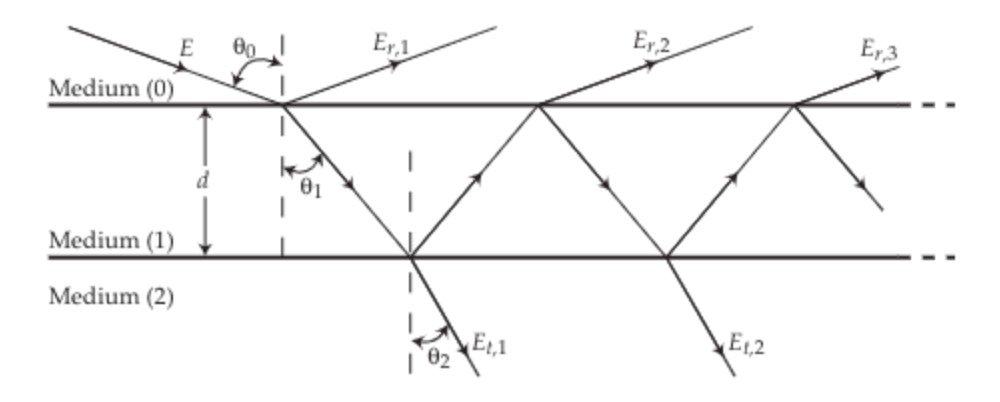
\includegraphics[scale=0.6]{three phase optical system.png} 
   \caption*{test}
\end{figure}


$E_{r,1...n}$ = reflected light \\
$E_{t,1...n}$ = transmitted light

$E_{r,1}$ has a phase change due to the propagation from $A$ to $E$ 
$E_{r,2}$ has a phase change due to the propagation from $A$ to $C$ 


\subsubsection*{Reflection and Transmission of an Incident Wave}
In a three phase system, an incident wave propagates through medium 0, 
and makes contact with medium 1 at an angle of \texttheta \textsubscript{0}. The incident wave is 
partially reflected at the boundary and partially transmitted through medium 1
at an angle of \texttheta \textsubscript{1}. The transmitted part of the incident wave
propagates through medium 1 until it makes contact with the boundary between medium 1 and 
medium 2. At this boundary the wave is again partially refelcted and partially transmitted
through medium 2 at an angle of \texttheta \textsubscript{2}. The connection between
thw angles \texttheta \textsubscript{0}, \texttheta \textsubscript{1} and
\texttheta \textsubscript{2} are given by Snell's law

\begin{equation}
    \tilde{n}_0 \sin( \theta_0) = \tilde{n}_1\sin(\theta_1)=\tilde{n}_2\sin(\theta_2)
\end{equation}
Where $\tilde{n}_0$, $\tilde{n}_1$ and $\tilde{n}_2$ are the complex refractive indxes for 
medium 0, 1 and 2 respectively.


\begin{subequations}
    \begin{align}
    & E_{r,1} = \rho_{01} \cdot E \\ 
    & E_{r, 2}=\tau_{01} e^{-j \beta} \rho_{12} e^{-j \beta} \tau_{10} \cdot E \\
    & E_{r, 3}=\tau_{01} e^{-j \beta} \rho_{12} e^{-j \beta} \rho_{10} e^{-j \beta} \rho_{12} e^{-j \beta} \tau_{10} \cdot E
    \end{align}
\end{subequations}



% \begin{gather} 
% \begin{align}
% |A D| &= \frac{|A E|}{2} \\
% |A B| &= \frac{|A B C|}{2}
% \end{align}
% \end{gather}

% \begin{equation}
%    |A D| = \frac{|A E|}{2} 
% \end{equation}

% \begin{equation}
%     |A B| = \frac{|A B C|}{2}
%  \end{equation}


% \begin{equation}
%     \boldsymbol{E}(z,t) = \boldsymbol{E_0}  \cos (\omega \cdot t - \boldsymbol{k} \cdot z + \varphi )
% \end{equation}


% \begin{align}
%     \beta &=\Phi_D-\Phi_B \\
%     &=\mathbf{k}_1 \cdot z_1-\mathbf{k}_{\mathbf{0}} \cdot z_0 \\
%     &=\frac{2 \pi}{\lambda}\left(\tilde{n}_1 \cdot z_1-\tilde{n}_0 \cdot z_0\right)
% \end{align}


% \begin{align}
%     z_1 &=\frac{d}{\cos \left(\theta_1\right)} \\
%     y &=\sin \left(\theta_1\right) \cdot z_1=\frac{d \cdot \sin \left(\theta_1\right)}{\cos \left(\theta_1\right)} \\
%     z_0 &=\sin \left(\theta_0\right) \cdot y=\frac{d \cdot \sin \left(\theta_1\right) \cdot \sin \left(\theta_0\right)}{\cos \left(\theta_1\right)}
% \end{align}

% \begin{equation}
%     \tilde{n}_0 = \frac{\tilde{n}_1 \cdot \sin(\theta_1)}{\sin (\theta_0)}
% \end{equation}


% \begin{align}
%     \beta &=\frac{2 \pi}{\lambda}\left(\tilde{n}_1 \cdot \frac{d}{\cos \left(\theta_1\right)}-\frac{\tilde{n}_1 \cdot \sin \left(\theta_1\right)}{\sin \left(\theta_0\right)} \cdot \frac{d \cdot \sin \left(\theta_0\right) \cdot \sin \left(\theta_1\right)}{\cos \left(\theta_1\right)}\right) \\
%     &=\frac{2 \pi \cdot d \cdot \tilde{n}_1}{\lambda}\left(\frac{1-\sin ^2\left(\theta_1\right)}{\cos \left(\theta_1\right)}\right) \\
%     &=2 \pi \frac{d}{\lambda} \tilde{n}_1 \cos \left(\theta_1\right) \\
%     &=2 \pi \frac{d}{\lambda} \sqrt{\tilde{n}_1^2-\tilde{n}_0^2 \sin ^2\left(\theta_0\right)}
% \end{align}


% \begin{equation}
%     P_n^{\prime}=\sum_{k=0}^n\left(\rho_{10} \rho_{12} e^{-j 2 \beta}\right)^k=1+\rho_{10} \rho_{12} e^{-j 2 \beta}+\rho_{10}^2 \rho_{12}^2 e^{-j 4 \beta}+\ldots+\left(\rho_{10} \rho_{12} e^{-j 2 \beta}\right)^n
% \end{equation}

% reset the counter
\setcounter{equation}{0}

% appendix section. * is used to suppress the section numbering
\section*{Appendix B. Hillock count code}

\begin{center}
\begin{boxedverbatim}
    OGName = getTitle();
fileName = replace(OGName, ".tif","");

run("Set Scale...", "distance=0.29113333 known=1 
pixel=1 unit=nm global"); 

path = getDirectory("image");

run("Bandpass Filter...", "filter_large=35 
filter_small=2 suppress=None tolerance=5 
autoscale saturate");

setAutoThreshold("Default dark");

//run("Threshold...");

run("Convert to Mask");

setThreshold(255, 255);

run("Analyze Particles...", "size=200.00-Infinity 
show=[Bare Outlines] 
display clear composite");

\end{boxedverbatim}
\end{center}
% reset the counter
\setcounter{equation}{0}

% appendix section. * is used to suppress the section numbering
\section*{Appendix C. Pinhole count code}

\begin{center}
\begin{boxedverbatim}
fileName = replace(OGName, ".png","");

run("Set Scale...", "distance=151.0915667 
known=1 pixel=1 unit=mm global"); 

path = getDirectory("image");

run("8-bit");

run("Bandpass Filter...", "filter_large=20 
filter_small=3 suppress=None tolerance=5 
autoscale saturate");

setAutoThreshold("Default dark");

//run("Threshold...");

run("Convert to Mask");

setThreshold(255, 255);

run("Analyze Particles...", "size=0-Infinity 
show=[Bare Outlines] display clear composite");
\end{boxedverbatim}
\end{center}

\end{document}
